%chktex-file 36
%chktex-file 23
%chktex-file 10
%chktex-file 17
%chktex-file 9
\documentclass[computationalMathematics.tex]{subfiles}

\begin{document}

%%%%%%%%%%%%%%~~~~~~~~~~~~~~~~~~~~~~~~~~~~~~~~~~~~~~~~%%%%%%%%%%%%%%%
\section{4th of October 2018 --- F. Poloni}
%%%%%%%%%%%%%%~~~~~~~~~~~~~~~~~~~~~~~~~~~~~~~~~~~~~~~~%%%%%%%%%%%%%%%

This lecture is about practical usage of the singular value decomposition and takes place almost wholly on Matlab.

For example, given a certain image, that can be represented as a matrix of values in the range $[0, 255]$, the rank-1 SVD of such image, results in a very abstract picture, see \Cref{fig:4ott_rank}.
The more we increase the rank, the better is the similarity of the approximated image with respect to the original one.

\syntax{
  Given a certain matrix $A$, we can compute the SVD decomposition using the command \texttt{[U, S, V] = svd(A)}
}


\begin{figure}[h]
  \centering
  \subfigure[Rank 1]{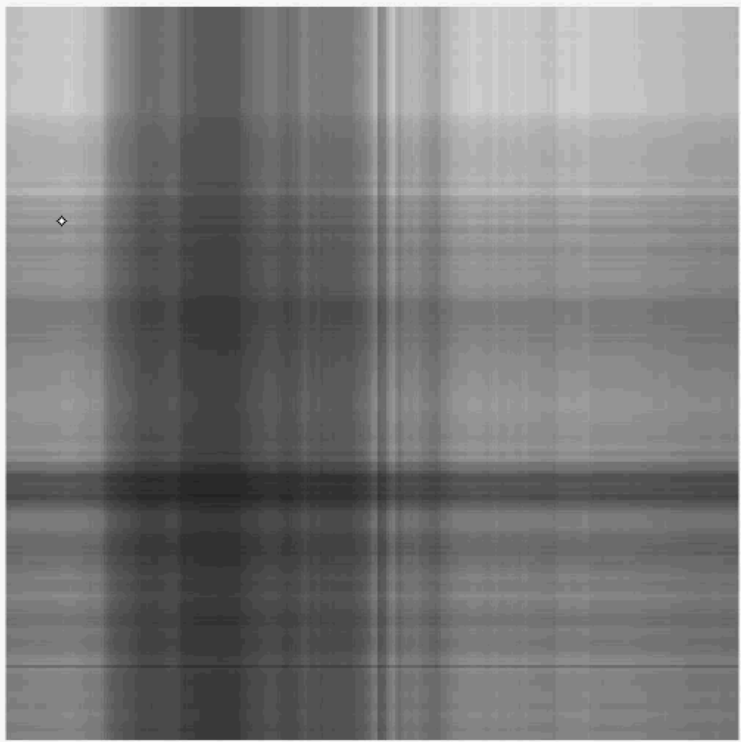
\includegraphics[width=0.35\textwidth]{pics/4ott/rank1.png}\label{subfloat:4ott_rk1}}
  \hspace{0.5cm}
  \subfigure[Rank 2]{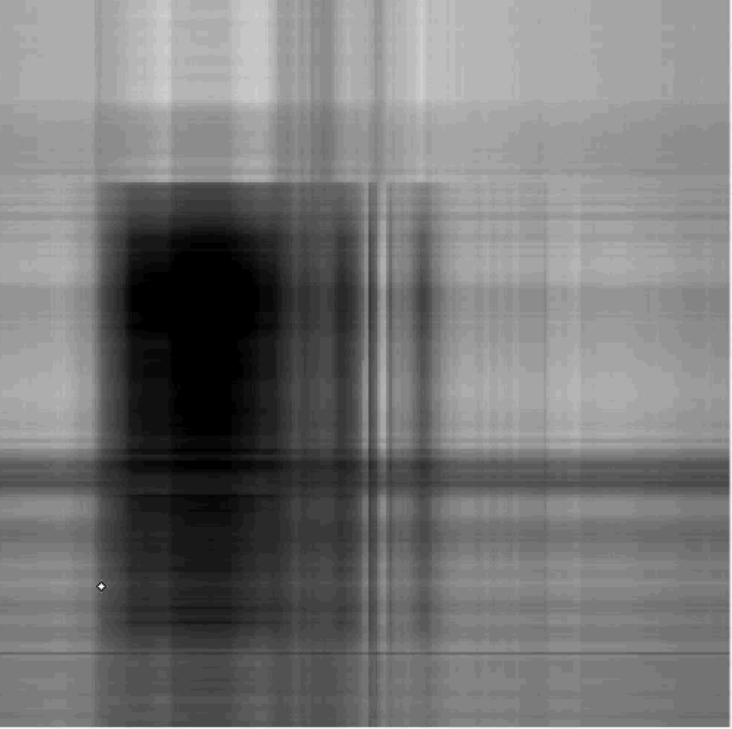
\includegraphics[width=0.35\textwidth]{pics/4ott/rank2.png}\label{subfloat:4ott_rk2}}\\
  \subfigure[Rank 5]{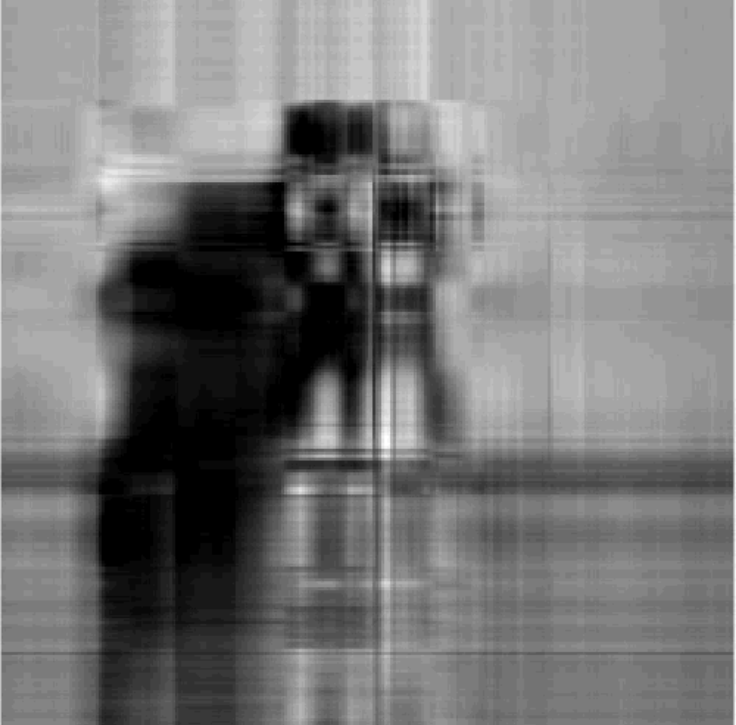
\includegraphics[width=0.35\textwidth]{pics/4ott/rank5.png}\label{subfloat:4ott_rk5}}
  \hspace{0.5cm}
  \subfigure[Full rank]{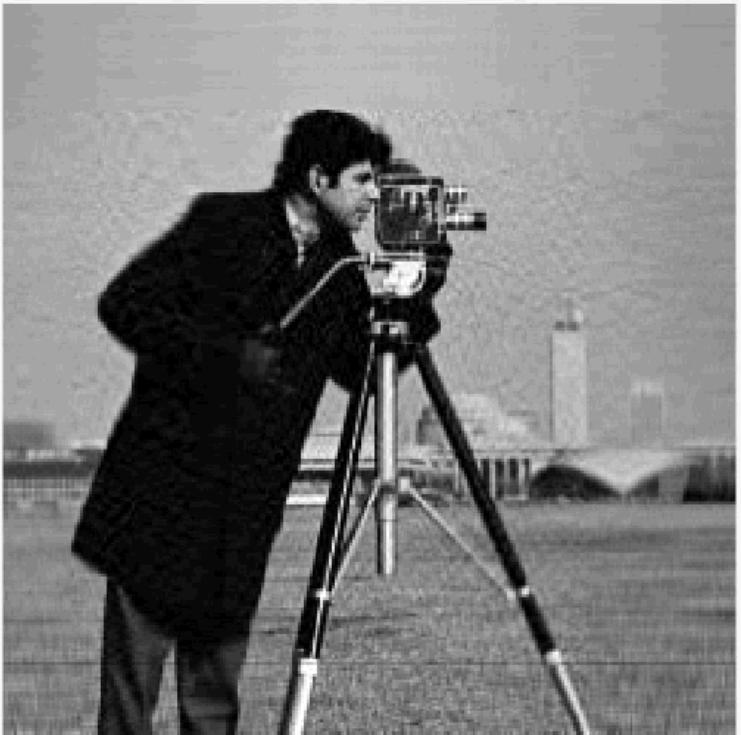
\includegraphics[width=0.35\textwidth]{pics/4ott/full_rank.png}\label{subfloat:4ott_rkfull}}\caption{How the approximation of a matrix changes with respect to the different ranks.}\label{fig:4ott_rank}
\end{figure}

\begin{definition}[Principal component analysis]
  Given a matrix $A$, we term \textbf{principal component analysis} the analysis of features of such matrix via the rows and columns of $U$ and $V$ respectively, where $U$ and $V$ are the matrices of the SVD decomposition.
\end{definition}


\end{document}
